\section{Resultados}
%
%\subsection{Códigos cíclicos não-BCH}
%
%\subsubsection{Polinômios geradores e distâncias mínimas}
%Os polinômios geradores utilizados e suas respectivas distâncias mínimas de código associado são mostradas em Listagem \ref{lst:polinomios}. Os índices são os mesmos do conjunto $S$ apresentado junto ao algoritmo. As distâncias mínimas, com mesma indexação de $S$, foram $\{2, 4, 3, 4, 2\}$.
%
%\begin{align}
%	\nonumber
%	p_1 = D^4+D^3+D^2+D+1\\ \nonumber
%	p_2 = D^5+D^3+D^2+1\\ \nonumber
%	p_3 = D^6+D^2+1\\ \nonumber
%	p_4 = D^6+D^4+D^3+D^2+1\\
%	p_5 = D^7+D^6+D^5+D^4+D^3+D^2+D+1
%	\label{lst:polinomios}
%\end{align}
%
%\subsubsection{Desempenho dos códigos cíclicos}
%
%Um gráfico comparativo entre os códigos aqui desenvolvidos e o código de Hamming é mostrado na Figura \ref{fig:cyclic_comparison}
%
%\begin{figure}[!hb]
%	\centering
%	\captionsetup{justification=centering}
%	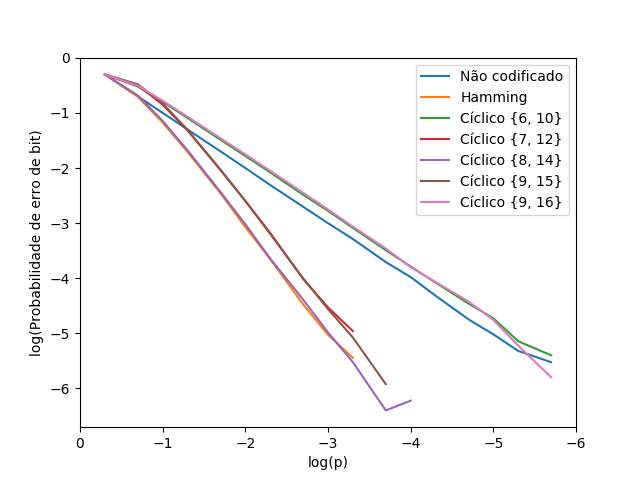
\includegraphics[scale=0.6]{floats/cyclic_5x10e6.png}
%	\caption{\label{fig:cyclic_comparison}Comparação da eficácia dos códigos cíclicos para 5004720 bits de informação enviados.}
%\end{figure}
%
%A título de comparação, a Figura \ref{fig:non_cyclic_comparison} traz os resultados do experimento anterior, o qual empregou códigos não necessariamente cíclicos obtidos pela tentativa de maximizar a distância mínima por meio de incrementos no tamanho de bloco.
%
%\begin{figure}[!hb]
%	\centering
%	\captionsetup{justification=centering}
%	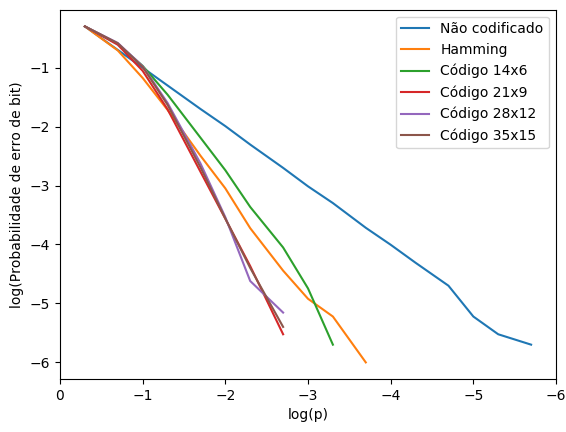
\includegraphics[scale=0.45]{floats/non_cyclic.png}
%	\caption{\label{fig:non_cyclic_comparison}Comparação da eficácia dos códigos não necessariamente cíclicos para 1000080 bits de informação enviados.}
%\end{figure}
%
%\subsection{Códigos BCH}
%
%\subsubsection{\label{complexidade_decod}Complexidade de decodificação BCH}
%
%Segundo \cite{ref:algoritmo-berlekamp}, a decodificação de códigos BCH se dá em $\mathcal{O}(n)$, $n$ sendo o tamanho de bloco empregado. Para confirmar a validade dessa afirmação, construíram-se códigos $BCH(m, 3)$, com $m \in \lbrace 4,5,...,20 \rbrace$, e mediram-se os tempos de decodificação submetendo a mesma palavra a cada um deles, com resultados ilustrados pela Figura \ref{fig:bch_decoding_is_linear}.
%
%\begin{figure}[!hb]
%	\centering
%    \captionsetup{justification=centering}
%	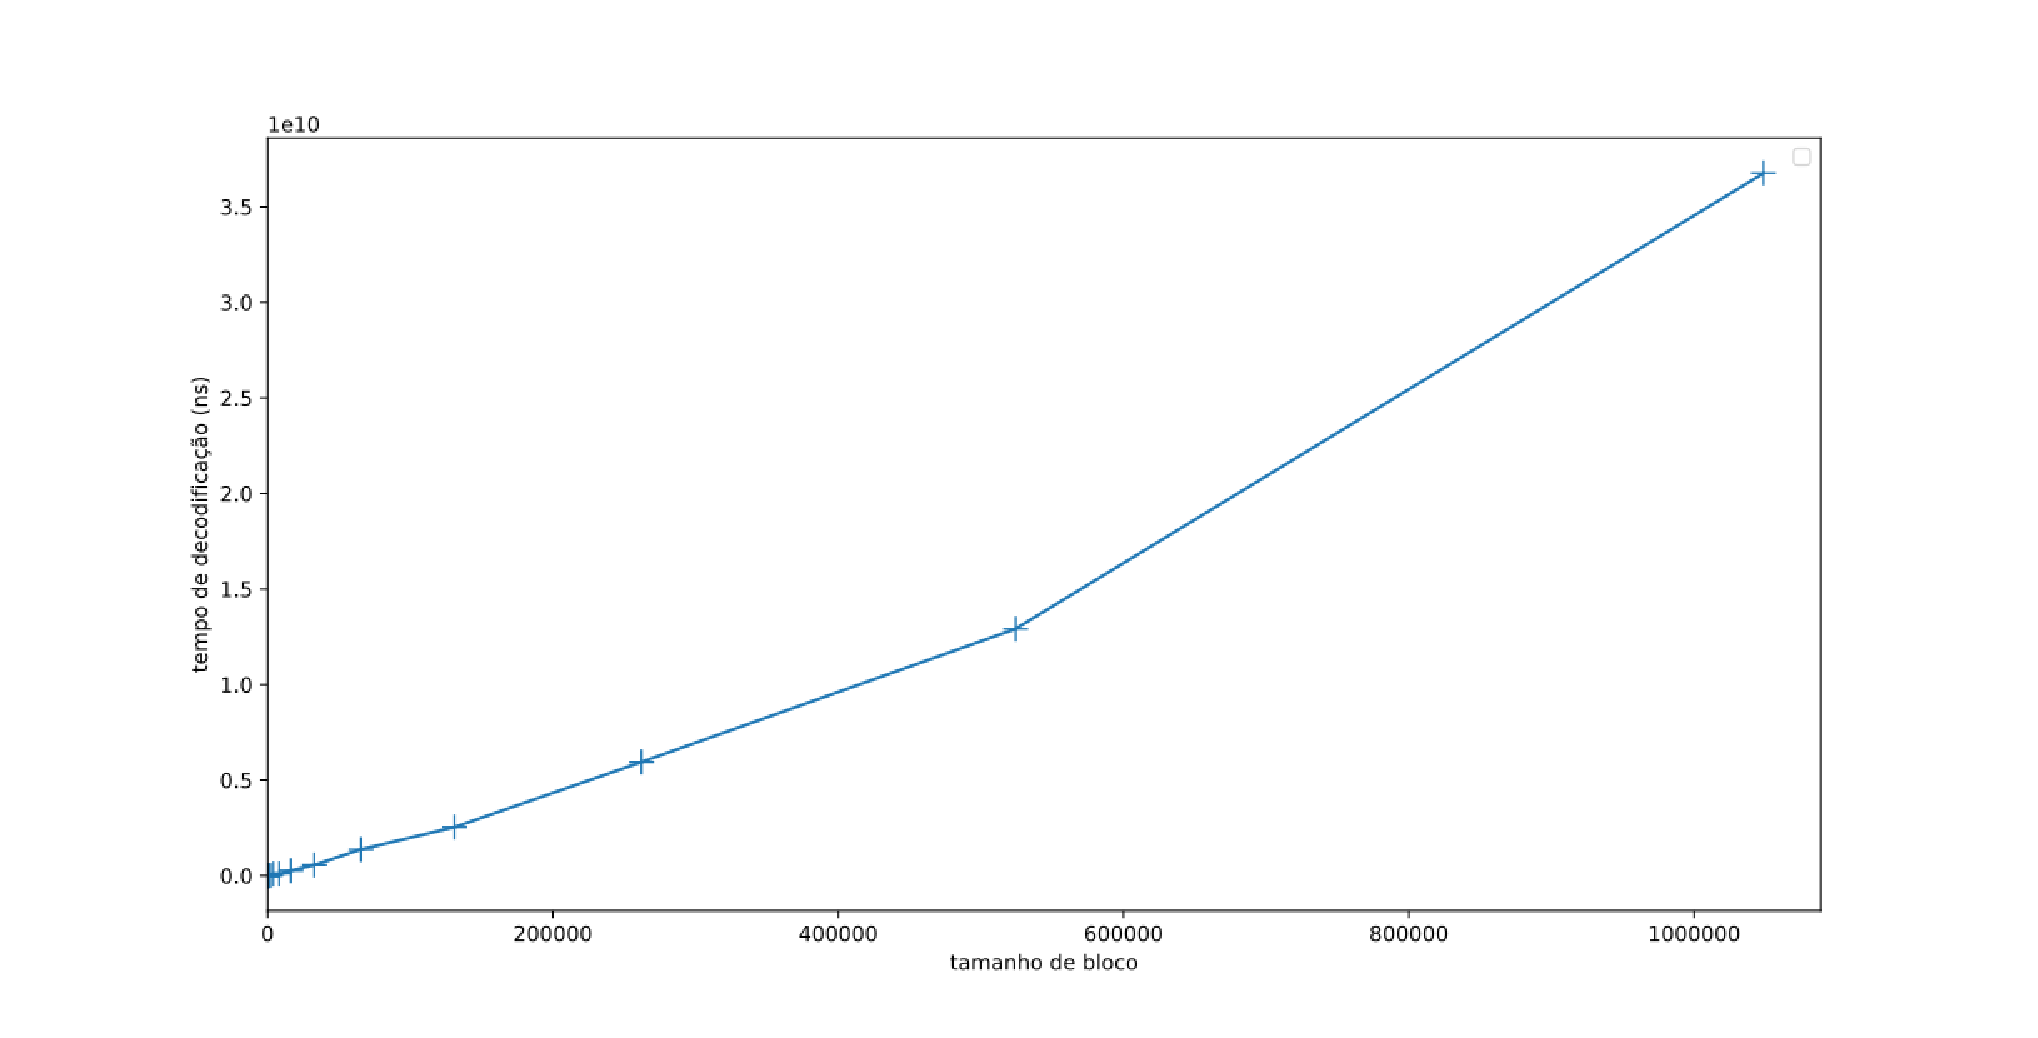
\includegraphics[scale=0.3]{floats/bch-decode-is-linear.eps}
%	\caption{\label{fig:bch_decoding_is_linear}Tempo de decodificação para BCH com variados tamanhos de bloco.}
%\end{figure}
%
%\subsubsection{\label{desempenho_bch}Desempenho do BCH}
%
%Para comparar o código BCH aos outros cíclicos, procurou-se um BCH de taxa próxima a 4/7 (usada como referência nos outros códigos deste laboratório), elegendo-se $BCH(5, 3)$ para ser submetido a testes sob canal BSC. A escolha se deu com base no polinômio gerador calculado, $g(X)=X^{15}+X^{11}+X^{10}+X^9+X^8+X^7+X^5+X^3+X^2+X+1$, que rendeu ao código taxa $\frac{31-15}{31}\simeq 0.52\simeq \frac{4}{7}\simeq 0.57$.
%
%Somente pela superior distância mínima projetada (3), era de se esperar que $BCH(5,3)$ superasse todos os outros códigos descritos neste texto. Isso é corroborado pela Figura \ref{fig:bch_performance}, na qual se vê que ele supera $Hamming(4,7)$ (que, por sua vez, tinha o mesmo desempenho aproximado dos outros códigos cíclicos).
%
%\begin{figure}[!hb]
%	\centering
%    \captionsetup{justification=centering}
%	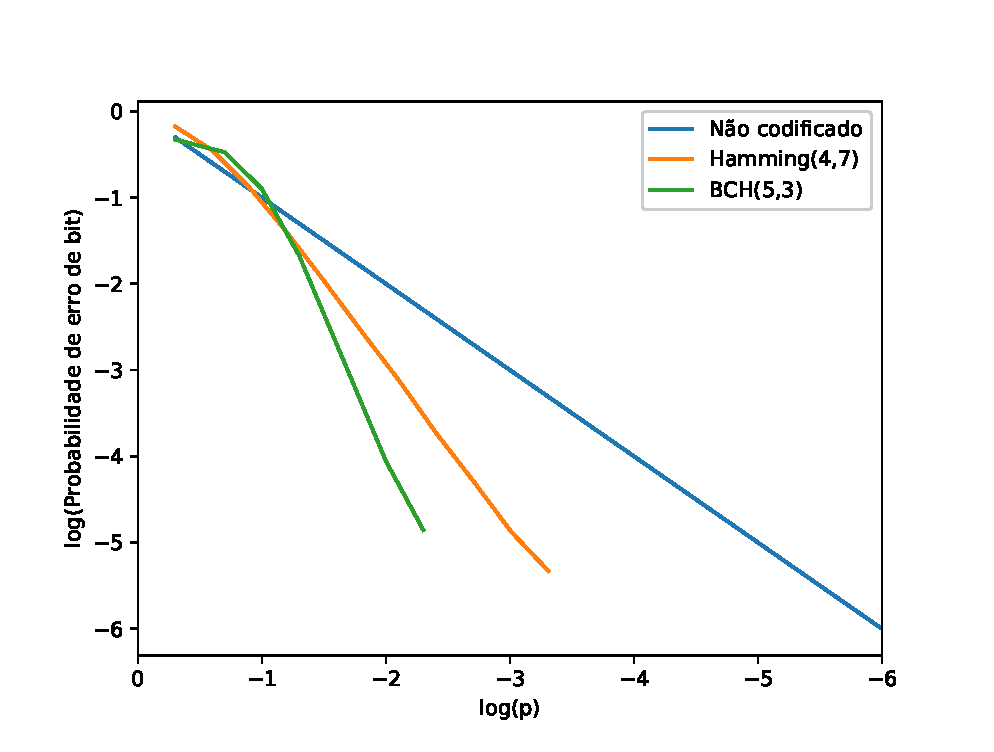
\includegraphics[scale=0.6]{floats/bch-performance.eps}
%	\caption{\label{fig:bch_performance}Chances de erro de bit de informação para $BCH(5,3)$ e $Hamming(4,7)$ sujeitos a canais BSC de variadas taxas de erro de bit.}
%\end{figure}